\documentclass{report}

\usepackage{hyperref}
\usepackage[
	newfloat=true,
]{minted}
\usepackage{caption}
\usepackage{float}
\usepackage[
	vmargin=1in,
	hmargin=1.5in,
]{geometry}
\usepackage{graphicx}
\usepackage{tabularx}
\usepackage{booktabs}
\usepackage[export]{adjustbox}
\usepackage[normalem]{ulem}
\usepackage{amsmath}
\usepackage{siunitx}

\hypersetup{
	colorlinks=true,
	linkcolor=blue,
}

\newenvironment{longlisting}{\captionsetup{type=listing}}{}
\newcommand{\floor}[1]{\left\lfloor #1 \right\rfloor}
\newcommand{\ceil}[1]{\left\lceil #1 \right\rceil}

\title{
	DM510 Operating systems \\
	Assignment 3 \\
	\normalsize File system \\
	\vspace{1cm}
	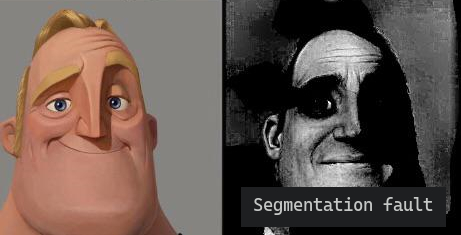
\includegraphics[width=0.99\textwidth, frame]{traummrinc}
}

\author{
	Frederik List \\
	\small frlis21@student.sdu.dk \\
}

\begin{document}

\maketitle

\section*{Introduction}

When booted, one of the first things operating systems do
is mount a block device, which probably has a file system on it.
One could hack the kernel to support a new file system, but that's hard.
FUSE lets us create a file system in userspace.
In this report, I outline how I created the terrible file system
(abbreviated TFS) with FUSE.

\section*{Design}

TFS is very barebones.
It can read and write (large) files and directories... and that's it.
TFS is neither journalling nor log structured.
The focus was on making TFS simple, which one might say TFS fails at,
for reasons you will discover.

\subsection*{Layout}

The layout of a TFS partition is as ordered:

\begin{itemize}
	\item TFS Superblock, containing
	      \begin{itemize}
		      \item the number of total blocks and nodes.
		      \item pointers to the heads of the free node and block linked lists.
	      \end{itemize}
	\item Nodes, where each node contains either
	      \begin{itemize}
		      \item node metadata, such as node name, blocks, access time, etc.
		      \item a pointer to the next free node in the free node linked list.
	      \end{itemize}
	\item Blocks, where each block contains either
	      \begin{itemize}
		      \item file data or directory entries.
		      \item indirect block pointers.
		      \item a single pointer to the next block in the free block linked list.
	      \end{itemize}
\end{itemize}

TFS allocates space for nodes near the beginning of the partition at format time.

\subsection*{Allocation scheme}

TFS uses a combined index allocation scheme
(exactly the one shown in figure 14.8 of the course textbook).
Early in development, TFS used a file allocation table (FAT) for its simplicity,
but the author suffers from occasional slight mental degradation and premature optimization syndrome,
so he chose to switch to the more complicated and slightly faster indexed allocation scheme.
(At least now he can open pictures of his dog a few milliseconds faster on a TFS mount.)

Random access is much faster for the indexed allocation scheme than for a FAT.
This is because instead of having to go through the entire file to find a specific block,
a formula can be used to calculate the block indices from the file offset.

If the required data cannot be found in the direct blocks,
then for a file block offset $x$
(starting at $0$ regardless of the number of direct blocks),
the indirect block level can be calculated with
\begin{align*}
	d = \floor{\log_b{\left( x + 1 - \floor{\frac{x + 1}{b}} \right)}}
\end{align*}
where $b =$ the number of block pointers that can fit in a block
($\frac{\text{block size}}{\text{pointer size}}$).
Block level indices can then be calculated with
\begin{align*}
	i_k = \floor{\frac{x - b \frac{b^d - 1}{b - 1}}{b^k}} \mod b
\end{align*}
where $k =$ index level.

If the block size (and block pointer size, and hence max block pointers) is a power of $2$,
then bit twiddling can be used for fast logarithm and exponent calculation.

\subsection*{Free nodes and blocks}

Free nodes contain a single pointer to the next free node,
thus forming a linked list of free nodes.

Similarly, free blocks contain a single pointer to the next free block.

\section*{Implementation}

TFS's code is somewhat littered with comments explaining most of the esoteric bits,
this section serves to supplement those comments.

\subsection*{Backing store}

TFS's backing store is in the form of a memory-mapped binary file.
A TFS image may be created with the provided \texttt{mktfs} utility,
much like Linux's \texttt{mke2fs(8)}.
As with \texttt{mke2fs}, a file needs to be allocated first,
probably with the \texttt{fallocate(1)} utility.
In the accompanying video a \qty{16}{MiB} file is allocated with \texttt{fallocate -l16M img.tfs},
after which \texttt{mktfs img.tfs} is invoked.

Instead of reading and writing to the file with, for example, \texttt{pread(2)},
TFS memory maps the entire backing store.
The author feels some might not think this to be in the spirit of the project,
but argues that without memory mapping, the code would just be polluted with
some extra \texttt{malloc}s and \texttt{pread}s.
Memory mapping allows everyone to enjoy the internals of TFS without more cruft than is required!

\subsection*{Looking up entries}

Entry lookup is implemented with the standard C library hash table
(see \texttt{hsearch(3)}).
Keys are paths and values are nodes.
This makes entry lookup very fast, but the memory usage may be a concern for large file systems,
as the hash table size is simply initialized to the number of nodes in the file system.

\subsection*{Reading and writing blocks}

An iterator-like structure named the ``block cursor''
allows for random-access seeking and sequential iteration.

Reading and writing are much the same.
A block cursor is simply set to the position to start from
and iterated until no more bytes can or should be written or read.

\subsection*{Allocating and freeing blocks and nodes}

Nodes are allocated and freed simply by popping from or pushing to the free node linked list.

Blocks are a little more tricky.
This is because in addition to blocks storing actual data,
index blocks also need to be allocated for sufficiently large files.
The cursor iterator presented earlier is able to take a callback ``hook''
which will be called for each block it iterates through,
including index blocks which are transparent to iterator consumers.

Allocation can be easily implemented using this callback.
A cursor is set to the end block of a file and iterated through
with a function that pops free blocks from the free block linked list.

Freeing blocks is not so easy.
Ideally, a cursor would be set to the end block of a file and iterated through \emph{backwards}
while freeing blocks along the way.
Instead, a hack was used that makes many assumptions about how the file system works:
a cursor is set to the last required block of a file and iterated,
adding any blocks along the way to a free block buffer.
After an iteration is done, any blocks in the free block buffer are freed
and the free block buffer is cleared.
This is not so good, as free block and index block pointers are written to the same locations,
and as the ancient proverb goes, ``don't shit where you eat''.

\section*{Crash recovery}

Crash recovery in TFS is nonexistent;
when the kernel decides to page out to the backing store is indeterminate.
Disregarding memory mapping, it could be implemented with journalling:
A portion of the TFS partition would be alloted to journalling,
where dirty blocks (and their checksums) would periodically be sequentially written.
After a journal is written, data can be moved to where it is supposed to go
with slower random access without fear of losing data.

In case of a crash, the journal can be read and the rearranging of data can be resumed.
Checksums are used to ensure only data that was successfully written to the journal
are written to the disk.

Journalling can handle any number of crashes while recovering from a crash;
the only data needed to recover is written to the nonvolatile disk.
Of course, some small amount of data loss is always possible when a crash occurs
while writing dirty blocks, the only remedy for which is to write often.

\section*{Tests}

Mosts of the tests performed in the video are just the author trying to abuse TFS as hard as he can.

\begin{figure}[h!]
	\caption{Tests with video timestamps}
	\centering
	\begin{tabularx}{12cm}{Xc}
		\toprule
		\textbf{Test}                                  & \textbf{Time} \\
		\midrule[1.5pt]
		Formatting                                     & 00:00         \\
		\midrule
		File creation and deletion                     & 00:10         \\
		\midrule
		Directory creation and deletion                & 00:24         \\
		\midrule
		Access and modification time using
		\texttt{touch} and \texttt{cat}                & 00:47         \\
		\midrule
		Large files using
		\texttt{seq}, \texttt{head}, and \texttt{tail} & 01:00         \\
		\midrule
		Directories with many entries                  & 01:12         \\
		\midrule
		good boi                                       & 01:29         \\
		\midrule
		File persistence                               & 01:39         \\
		\bottomrule
	\end{tabularx}
\end{figure}

In more rigorous testing under development,
an ad-hoc analysis concluded that TFS does not produce dead blocks or leak memory.

TFS breaks down a little bit when there is not much space left.
Not all cases concerning lack of storage are well tested.

\section*{Conclusion}

Though the author would not trust it for anything remotely important, it works.
TFS is slow and probably riddled with nasty bugs,
but it gets the job done.

\appendix

\chapter{Source code}

\setminted{
	numbers=left,
	fontsize=\footnotesize,
	tabsize=8,
	obeytabs=true,
}

\begin{longlisting}
	\caption{\texttt{tfs.h}}
	\label{lst:tfsh}
	\inputminted{c}{../tfs.h}
\end{longlisting}

\begin{longlisting}
	\caption{\texttt{fuse\_tfs.c}}
	\label{lst:fuse}
	\inputminted{c}{../fuse_tfs.c}
\end{longlisting}

\begin{longlisting}
	\caption{\texttt{tfs.c}}
	\label{lst:tfs}
	\inputminted{c}{../tfs.c}
\end{longlisting}

\begin{longlisting}
	\caption{\texttt{mktfs.c}}
	\label{lst:mktfs}
	\inputminted{c}{../mktfs.c}
\end{longlisting}

\end{document}
